% --------------------------------------------------------------
% This is all preamble stuff that you don't have to worry about.
% Head down to where it says "Start here"
% --------------------------------------------------------------
 
\documentclass[12pt]{article}
 
\usepackage[margin=1in]{geometry} 
\usepackage{amsmath,amsthm,amssymb,scrextend}
\usepackage{fancyhdr}
\usepackage{enumitem}
\usepackage{amsmath}
\usepackage{amssymb}
\usepackage{textcomp}
\usepackage{fancybox}
\usepackage{tikz}
\usepackage{tasks}
\pagestyle{fancy}
\usepackage[makeroom]{cancel}
\usepackage{graphicx}
\usepackage{caption}
\usepackage{mwe}
\usepackage{tikz}
\usetikzlibrary{positioning}

\newcommand{\N}{\mathbb{N}}
\newcommand{\Z}{\mathbb{Z}}
\newcommand{\I}{\mathbb{I}}
\newcommand{\R}{\mathbb{R}}
\newcommand{\Q}{\mathbb{Q}}
\renewcommand{\qed}{\hfill$\blacksquare$}
\let\newproof\proof
\renewenvironment{proof}{\begin{addmargin}[1em]{0em}\begin{newproof}}{\end{newproof}\end{addmargin}\qed}
% \newcommand{\expl}[1]{\text{\hfill[#1]}$}
 
\newenvironment{theorem}[2][Theorem]{\begin{trivlist}
\item[\hskip \labelsep {\bfseries #1}\hskip \labelsep {\bfseries #2.}]}{\end{trivlist}}
\newenvironment{lemma}[2][Lemma]{\begin{trivlist}
\item[\hskip \labelsep {\bfseries #1}\hskip \labelsep {\bfseries #2.}]}{\end{trivlist}}
\newenvironment{problem}[2][Problem]{\begin{trivlist}
\item[\hskip \labelsep {\bfseries #1}\hskip \labelsep {\bfseries #2.}]}{\end{trivlist}}
\newenvironment{exercise}[2][Exercise]{\begin{trivlist}
\item[\hskip \labelsep {\bfseries #1}\hskip \labelsep {\bfseries #2.}]}{\end{trivlist}}
\newenvironment{reflection}[2][Reflection]{\begin{trivlist}
\item[\hskip \labelsep {\bfseries #1}\hskip \labelsep {\bfseries #2.}]}{\end{trivlist}}
\newenvironment{proposition}[2][Proposition]{\begin{trivlist}
\item[\hskip \labelsep {\bfseries #1}\hskip \labelsep {\bfseries #2.}]}{\end{trivlist}}
\newenvironment{corollary}[2][Corollary]{\begin{trivlist}
\item[\hskip \labelsep {\bfseries #1}\hskip \labelsep {\bfseries #2.}]}{\end{trivlist}}
 
\setlength{\parindent}{0pt}
\begin{document}
 \settasks{
	counter-format=(tsk[r]),
	label-width=4ex
}
% --------------------------------------------------------------
%                         Start here
% --------------------------------------------------------------

\lhead{Math 475}
\chead{Homework 2}
\rhead{Meenmo Kang}

\begin{itemize}
    \item[\bf 2.7.16] Prove that $$\binom{n}{r}=\binom{n}{n-r}$$ by using a combinatorial argument and not the values of these numbers as given in Theorem 3.3.1. 
    
    $$\binom{n}{r}= \frac{n!}{(n-r)!r!}=\frac{n!}{(n-r)!(n-(n-r))!} = \binom{n}{n-r}$$\\
    
    
    \item[\bf 2.7.17] 
    \begin{itemize}
        \item In how many ways can six indistinguishable rooks be placed on a 6-by-6 board so that no two rooks can attack one another? $6!$\\
        
        There should be only one rook in any row or column not to be attacked by another rook. Suppose we place the first rook. There are six options at first. Then, when we place the second one, there are five options excluding the row/column that is shared by the first one. Therefore, the number of possible ways is 6!.\\
        
        \item In how many ways if there are two red and four blue rooks? $\binom{6}{2}\cdot 6!$\\
        
        The approach for placing rooks is same, but since they are distinguishable now, we need to consider the arrangement of them by two color. Therefore, we can just multiply 6! by $\binom{6}{2}$.
    \end{itemize} 
    
    \vspace{2\baselineskip}
    \item[\bf 2.7.18] In how many ways can two red and four blue rooks be placed on an 8-by-8 board so that no two rooks can attack one another?\\
    
    Suppose we are choosing columns to locate the two red rooks. The number of ways of this is $\binom{8}{2}$. As for rows, we have 8 options for the first red rook and 7 options for the second red rook. Similarly, the number of ways of choosing columns to place the four blue rooks is $\binom{8-2}{4}$ and 6,5,4,3 options for rows respectively. Thus, the answer for this question is $\binom{8}{2}\cdot8\cdot 7 + \binom{6}{4}\cdot 6\cdot 5\cdot 4\cdot 3$.
    
    \vspace{2\baselineskip}
    \item[\bf 2.7.21] How many permutations are there of the letters of the word ADDRESSES? How many 8-permutations are there of these nine letters?\\
    
    $$\underbrace{\binom{9}{1}}_{1\; A}\cdot \underbrace{\binom{8}{2}}_{2\; D}\cdot \underbrace{\binom{6}{1}}_{1\;R}\cdot \underbrace{\binom{5}{3}}_{3\;S}\cdot \underbrace{\binom{2}{2}}_{2\;E}$$
    
    \item[\bf 2.7.28] A secretary works in a building located nine blocks east and eight blocks north of his home. Every day he walks 17 blocks to work. (See the map that follows.)
    
    \begin{center}
        \tikzset{every picture/.style={line width=0.75pt}} %set default line width to 0.75pt        
        
        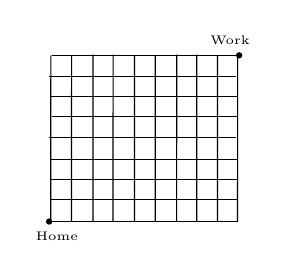
\begin{tikzpicture}[x=0.75pt,y=0.75pt,yscale=-1,xscale=1]
        %uncomment if require: \path (0,423.0242919921875); %set diagram left start at 0, and has height of 423.0242919921875
        
        %Straight Lines [id:da005306609169222876] 
        \draw    (99.93,120.14) -- (99.89,200.21) ;
        
        
        %Straight Lines [id:da6341048293198255] 
        \draw    (109.93,120.14) -- (109.89,200.21) ;
        
        
        %Straight Lines [id:da8468042261170148] 
        \draw    (120.26,119.81) -- (120.23,199.88) ;
        
        
        %Straight Lines [id:da6689694696995792] 
        \draw    (129.93,119.81) -- (129.89,199.88) ;
        
        
        %Straight Lines [id:da5913811345883242] 
        \draw    (140.26,120.14) -- (140.23,200.21) ;
        
        
        %Straight Lines [id:da486851972039398] 
        \draw    (150.26,120.14) -- (150.23,200.21) ;
        
        
        %Straight Lines [id:da9933104615474264] 
        \draw    (160.6,119.81) -- (160.56,199.88) ;
        
        
        %Straight Lines [id:da4165314325550753] 
        \draw    (170.26,119.81) -- (170.23,199.88) ;
        
        
        %Straight Lines [id:da1703915562343472] 
        \draw    (180.26,120.14) -- (180.23,200.21) ;
        
        
        %Straight Lines [id:da1313356409587194] 
        \draw    (189.93,120.14) -- (189.89,200.21) ;
        
        
        %Straight Lines [id:da3338321916113951] 
        \draw    (100.26,120.14) -- (190.26,120.14) ;
        
        
        %Straight Lines [id:da2457669685488637] 
        \draw    (99.26,130.14) -- (189.26,130.14) ;
        
        
        %Straight Lines [id:da042291165965059996] 
        \draw    (99.93,139.81) -- (189.93,139.81) ;
        
        
        %Straight Lines [id:da048211808106058296] 
        \draw    (100.26,149.81) -- (190.26,149.81) ;
        
        
        %Straight Lines [id:da22775227194247805] 
        \draw    (99.26,159.81) -- (189.26,159.81) ;
        
        
        %Straight Lines [id:da11917894314252209] 
        \draw    (99.93,189.48) -- (189.93,189.48) ;
        
        
        %Straight Lines [id:da49931816470901613] 
        \draw    (99.93,170.14) -- (189.93,170.14) ;
        
        
        %Straight Lines [id:da48502334543496084] 
        \draw    (99.93,180.14) -- (189.93,180.14) ;
        
        
        %Straight Lines [id:da9944653422610548] 
        \draw    (99.89,200.21) -- (189.89,200.21) ;
        
        %Flowchart: Connector [id:dp7556158148444003] 
        \draw  [fill={rgb, 255:red, 0; green, 0; blue, 0 }  ,fill opacity=1 ] (97.89,200.21) .. controls (97.89,199.53) and (98.45,198.97) .. (99.14,198.97) .. controls (99.83,198.97) and (100.39,199.53) .. (100.39,200.21) .. controls (100.39,200.9) and (99.83,201.46) .. (99.14,201.46) .. controls (98.45,201.46) and (97.89,200.9) .. (97.89,200.21) -- cycle ;
        %Flowchart: Connector [id:dp3697063794071094] 
        \draw  [fill={rgb, 255:red, 0; green, 0; blue, 0 }  ,fill opacity=1 ] (189.43,120.14) .. controls (189.43,119.46) and (189.99,118.9) .. (190.68,118.9) .. controls (191.37,118.9) and (191.93,119.46) .. (191.93,120.14) .. controls (191.93,120.83) and (191.37,121.38) .. (190.68,121.38) .. controls (189.99,121.38) and (189.43,120.83) .. (189.43,120.14) -- cycle ;
        
        % Text Node
        \draw (102.89,207.21) node [scale=0.9] [align=left] {{\tiny Home}};
        % Text Node
        \draw (186.35,112.9) node [scale=0.9] [align=left] {{\tiny Work}};
        \end{tikzpicture}
    \end{center}
    
    \begin{enumerate}[label=(\alph*)]
        \item How many different routes are possible for him?\\
        
        He walks 17 blocks to work from home, but he is walking towards only east or north. So, we can think simply this problem as arranging 8 {\bf N} (for north) and 9 {\bf E} (for east) in 17 blanks. Hence, the answer is $$\binom{17}{8} \text{ or } \binom{17}{9}$$\\
        
        \item How many different routes are possible if the one block in the easterly direction, which begins four blocks east and three blocks north of his home, is under water (and he can't swim)? (Hint: Count the routes that use the block under water.)
        
        \begin{center}
        \tikzset{every picture/.style={line width=0.75pt}} %set default line width to 0.75pt        
        
        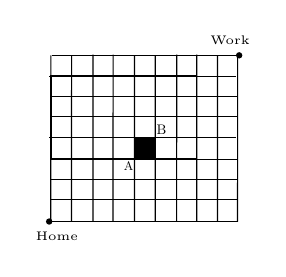
\begin{tikzpicture}[x=0.75pt,y=0.75pt,yscale=-1,xscale=1]
        %uncomment if require: \path (0,423.0242919921875); %set diagram left start at 0, and has height of 423.0242919921875
        
        %Straight Lines [id:da005306609169222876] 
        \draw    (99.93,120.14) -- (99.89,200.21) ;
        
        
        %Straight Lines [id:da6341048293198255] 
        \draw    (109.93,120.14) -- (109.89,200.21) ;
        
        
        %Straight Lines [id:da8468042261170148] 
        \draw    (120.26,119.81) -- (120.23,199.88) ;
        
        
        %Straight Lines [id:da6689694696995792] 
        \draw    (129.93,119.81) -- (129.89,199.88) ;
        
        
        %Straight Lines [id:da5913811345883242] 
        \draw    (140.26,120.14) -- (140.23,200.21) ;
        
        
        %Straight Lines [id:da486851972039398] 
        \draw    (150.26,120.14) -- (150.23,200.21) ;
        
        
        %Straight Lines [id:da9933104615474264] 
        \draw    (160.6,119.81) -- (160.56,199.88) ;
        
        
        %Straight Lines [id:da4165314325550753] 
        \draw    (170.26,119.81) -- (170.23,199.88) ;
        
        
        %Straight Lines [id:da1703915562343472] 
        \draw    (180.26,120.14) -- (180.23,200.21) ;
        
        
        %Straight Lines [id:da1313356409587194] 
        \draw    (189.93,120.14) -- (189.89,200.21) ;
        
        
        %Straight Lines [id:da3338321916113951] 
        \draw    (100.26,120.14) -- (190.26,120.14) ;
        
        
        %Straight Lines [id:da2457669685488637] 
        \draw    (99.26,130.14) -- (189.26,130.14) ;
        
        
        %Straight Lines [id:da042291165965059996] 
        \draw    (99.93,139.81) -- (189.93,139.81) ;
        
        
        %Straight Lines [id:da048211808106058296] 
        \draw    (100.26,149.81) -- (190.26,149.81) ;
        
        
        %Straight Lines [id:da22775227194247805] 
        \draw    (99.26,159.81) -- (189.26,159.81) ;
        
        
        %Straight Lines [id:da11917894314252209] 
        \draw    (99.93,189.48) -- (189.93,189.48) ;
        
        
        %Straight Lines [id:da49931816470901613] 
        \draw    (99.93,170.14) -- (189.93,170.14) ;
        
        
        %Straight Lines [id:da48502334543496084] 
        \draw    (99.93,180.14) -- (189.93,180.14) ;
        
        
        %Straight Lines [id:da9944653422610548] 
        \draw    (99.89,200.21) -- (189.89,200.21) ;
        
        
        %Flowchart: Connector [id:dp7556158148444003] 
        \draw  [fill={rgb, 255:red, 0; green, 0; blue, 0 }  ,fill opacity=1 ] (97.89,200.21) .. controls (97.89,199.53) and (98.45,198.97) .. (99.14,198.97) .. controls (99.83,198.97) and (100.39,199.53) .. (100.39,200.21) .. controls (100.39,200.9) and (99.83,201.46) .. (99.14,201.46) .. controls (98.45,201.46) and (97.89,200.9) .. (97.89,200.21) -- cycle ;
        %Flowchart: Connector [id:dp3697063794071094] 
        \draw  [fill={rgb, 255:red, 0; green, 0; blue, 0 }  ,fill opacity=1 ] (189.43,120.14) .. controls (189.43,119.46) and (189.99,118.9) .. (190.68,118.9) .. controls (191.37,118.9) and (191.93,119.46) .. (191.93,120.14) .. controls (191.93,120.83) and (191.37,121.38) .. (190.68,121.38) .. controls (189.99,121.38) and (189.43,120.83) .. (189.43,120.14) -- cycle ;
        %Shape: Rectangle [id:dp37962460269714704] 
        \draw   (100,130) -- (170,130) -- (170,170) -- (100,170) -- cycle ;
        %Shape: Rectangle [id:dp06707621007414333] 
        \draw  [fill={rgb, 255:red, 0; green, 0; blue, 0 }  ,fill opacity=1 ] (140.24,160.18) -- (149.67,160.18) -- (149.67,169.7) -- (140.24,169.7) -- cycle ;
        
        % Text Node
        % Text Node
        \draw (102.89,207.21) node [scale=0.9] [align=left] {{\tiny Home}};
        % Text Node
        \draw (186.35,112.9) node [scale=0.9] [align=left] {{\tiny Work}};
        % Text Node
        \draw (137.43,173.51) node [scale=0.5] [align=left] {{\small A}};
        % Text Node
        \draw (153.24,156.18) node [scale=0.5] [align=left] {B};
        \end{tikzpicture}
        \end{center}
        
        Similarly, in this case, we can divide into two cases: 
        \begin{itemize}
            \item Home $\rightarrow$ A: $\binom{7}{3}$ or $\binom{7}{4}$
            
            \item B $\rightarrow$ Work: $\binom{8}{4}$
        \end{itemize}
        
        Hence the answer is 
        $$\binom{17}{8}-\binom{7}{4} \cdot \binom{8}{4}$$
    \end{enumerate}
    
    \newpage
    \item[\bf 2.7.32] Determine the number of 11-permutations of the multiset
    $$S=\{3\cdot a,\; 4\cdot b,\;5\cdot c\}$$
    
    \begin{enumerate}[label=(\roman*)]
        \item Excluding one $a$
        $$\binom{11}{2}\cdot\binom{9}{4}\cdot\binom{5}{5}$$
        
        \item Excluding one $b$
        $$\binom{11}{3}\cdot\binom{8}{3}\cdot\binom{5}{5}$$
        
        \item Excluding one $c$
        $$\binom{11}{3}\cdot\binom{8}{4}\cdot\binom{4}{4}$$
    \end{enumerate}
    
    The answer is (i)+(ii)+(iii).\\
    
    \item[\bf 2.7.35] List all 3-combinations and 4-combinations of the multiset 
    $$\{2\cdot a,\; 1\cdot b,\; 3\cdot c\}$$
    
    \begin{itemize}
        \item All 3-combinations
        $$\{a,a,b\},\{a,a,c\},\{a,b,c\},\{a,c,c\},\{b,c,c\},\{c,c,c\}$$
        \item All 4-combinations
        $$\{a,a,b,c\},\{a,a,c,c\},\{a,b,c,c\},\{a,c,c,c\},\{b,c,c,c\}$$
    \end{itemize}
    
    \item[\bf 2.7.37] A bakery sells six different kinds of pastry.
    \begin{itemize}
        \item If the bakery has at least a dozen of each kind, how many different options for a dozen of pastries are there?\\
        
        The number of different options for boxes equals the number of 12-combinations of a multiset with objects of 6 types, each having an (technically) infinite repetition number. Hence, by theorem 2.5.1 on the textbook, we can deduce the answer of this question as below.
        $$\binom{12+6-1}{12}$$\\
        
        \item What if a box is to contain at least one of each kind of pastry?\\
        
        Fix the six pastries which are one of each kind of pastry. Then we can do same computation with remaining six spots.
        $$\binom{6+6-1}{6}$$
    \end{itemize} 
    
    \item[\bf 2.7.38] How many integral solutions of
    $$x_1+x_2+x_3+x_4 = 30$$
    satisfy $x_1\ge 2,\; x_2\ge 0,\; x_3\ge -5,$ and $x_4\ge 8$?\\
    
    Let $y_1 = x_1-2,\; y_3 = x_3+5,\text{ and } y_4 = x_4-8$. Then $y_1+y_2+y_3+y_4=25,$ and all $y_i$ are non-negative integers (where $1\le i\le 4$). Using the Theorem 2.5.1 again (since this is about multiset with four different types), the answer is achieved as follows.
    $$\binom{25+4-1}{25}$$
    
    \item[\bf 2.7.42] Determine the number of ways to distribute 10 orange drinks, 1 lemon drink, and 1 lime drink to four thirsty students so that each student gets at least one drink, and the lemon and lime drinks go to different students.\\
    
    Suppose lemon and lime drinks are given to different students. The possible number of this cases is $4\times 3=12$. Since every students should have at least one drink, suppose each orange drinks is distributed to two students who do not have any drink yet. Then this became the problem of multiset with four different types since 8 orange drinks have to be distributed to four people. Therefore, the answer is $$12\cdot \binom{8+4-1}{8}$$
    
    \item[\bf 2.7.45] Twenty different books are to be put on five book shelves, each of which holds at least twenty books.
    \begin{enumerate}[label=(\alph*)]
        \item How many different arrangements are there if you only care about the number of books on the shelves (and not which book is where)?
        $$\binom{20+5-1}{5-1}$$
        
        \item How many different arrangements are there if you care about which books are where, but the order of the books on the shelves doesn't matter?
        $$5^{20}$$
        
        \item How many different arrangements are there if the order on the shelves does matter?
        $$\binom{20+5-1}{5-1}\cdot 20!$$
    \end{enumerate}
    
    \newpage
    \item[\bf 2.7.60] A bagel store sells six different kinds of bagels. Suppose you choose 15 bagels at random. 
    
    \begin{itemize}
        \item What is the probability that your choice contains at least one bagel of each kind?\\
        
        We can follow exactly same approach that is used for the question \textbf{2.7.37}.
        $$\frac{\binom{(15-6)+6-1}{15-6}}{\binom{15+6-1}{15}}=\frac{\binom{14}{9}}{\binom{20}{15}}$$
        
        \item If one of the kinds of bagels is Sesame, what is the probability that your choice contains at least three Sesame bagels?
        $$1-\frac{\overbrace{\binom{15+5-1}{15}}^{0\; Sesame}+\overbrace{\binom{(15-1)+5-1}{15-1}}^{1\;Sesame}+\overbrace{\binom{(15-2)+5-1}{15-2}}^{2\;Sesame}}{\binom{20}{15}}$$
    \end{itemize}
     \\
    
    \item[\bf 2.7.63] Four (standard) dice (cubes with 1, 2, 3, 4, 5, 6, respectively, dots on their six faces), each of a different color, are tossed, each landing with one of its faces up, thereby showing a number of dots. Determine the following probabilities:
    \begin{enumerate}[label=(\alph*)]
        \item The probability that the total number of dots shown is 6\\
        
        All possible sets whose sum is 6 is
        $$\{1,1,1,3\},\{1,1,2,2\},\{1,1,3,1\},\{1,2,1,2\},\{1,1,2,1\},$$
        $$\{1,3,1,1\},\{2,1,1,2\},\{2,1,2,1\},\{2,2,1,1\},\{3,1,1,1\}$$
        
        Hence the answer is $$\frac{10}{6^4}$$
        \item The probability that at most two of the dice show exactly one dot
        $$\frac{\overbrace{5^4}^{No\; 1}+ \overbrace{\binom{4}{1}\cdot 5^3\cdot 1^1}^{One\; 1}+ \overbrace{\binom{4}{2}\cdot 5^2\cdot 1^2}^{Two\; 1}}{6^4}$$\\
        
        \item The probability that each die shows at least two dots
        $$\left(\frac{5}{6}\right)^4$$
        \item The probability that the four numbers of dots shown are all different
        $$\frac{\binom{6}{1}\cdot\binom{5}{1}\cdot\binom{4}{1}\cdot\binom{3}{1}}{6^4}$$
        \item The probability that there are exactly two different numbers of dots shown\\
        $$\frac{\overbrace{\binom{6}{1}\cdot \binom{5}{1}\cdot \binom{4}{3}}^{\text{3 dice of one number}} + \overbrace{\binom{6}{2}\cdot\binom{4}{2}}^{\text{2 dice of one number}}}{6^4}$$
    \end{enumerate}
    
\end{itemize}
\end{document}